%Part of/Parte di https://github.com/f-dinucci/appuntiMeccanicaFluidi/
%License/Licenza Creative Commons Attribution-ShareAlike 4.0 International (CC BY-SA 4.0) - attribution/attribuzione Francesco Di Nucci
%See also/Vedere anche https://creativecommons.org/licenses/by-sa/4.0/ and/e https://creativecommons.org/licenses/by-sa/4.0/legalcode
%
\section{Profili di velocità}  
%SUBSECTION
\subsection{Profili di velocità}
Non è possibile trovare il profilo di velocità a partire dalle equazioni, dato che ci sono più incognite che equazioni.
È necessario legare velocità e $\tau_w$ (sforzo alla parete) con un cosiddetto modello di turbolenza, nel caso delle pareti parallele di un condotto ci si può arrivare tramite l'adimensionalizzazione.

Innanzitutto si può ridurre il numero di parametri di cui è funzione la velocità.
Nel defect layer la viscosità è trascurabile:
%
	\begin{equation*}
		u = u(y, h, \nu, \tau_w) = u(y, h, \tau_w)
	\end{equation*}
%
Il wall layer è sottile, solo vicino alla parete è dominato dallo sforzo viscoso, è piccolo, h trascurabile:
%
	\begin{equation*}
		u = u(y, h, \nu, \tau_w) = u(y, \nu, \tau_w)
	\end{equation*}
%
Lo sforzo totale è dato da (per simmetria $C= 0$):
%
	\begin{equation*}
		\tau_w = - h p_x
	\end{equation*}
%
Viene poi trasformato tramite una velocità di riferimento (shear velocity/velocità di taglio)
%
	\begin{equation*}
		u_\tau = \sqrt{\frac{\tau_w}{\rho} }
	\end{equation*}
%
Questa indica l'ordine di grandezza delle fluttuazioni di velocità, le fluttuazioni risultano essere di poco più piccole della velocità media.

Adimensionalizzando i profili di velocità per ridurre il numero di variabili diventano funzioni del tipo:
%
	\begin{equation*}
		\begin{gathered}
			\text{defect layer}\\
			\frac{u}{u_\tau} = F \left( \frac{y}{h} \right)\\
			\text{wall layer}\\
			\frac{u}{u_\tau} = f\left( \frac{y u_\tau}{\nu} \right)
		\end{gathered}
	\end{equation*}
%
È utile separarli perché altrimenti si avrebbe $\frac{u}{u_\tau} = G\left( \frac{y}{h}, \frac{y u_t}{\nu} \right)$, che è una funzione di due variabili.

Nel defect layer si ragiona rispetto alla velocità massima, si definisce quindi il difetto di velocità/velocity defect che dà il nome allo strato come differenza tra la velocità massima e quella in un punto generico:
%
	\begin{equation*}
		\begin{gathered}
			\frac{U - u}{u_\tau} \quad \text{Velocity defect}\\
			\frac{U - u}{u_\tau} = \frac{U}{u_\tau} - F \left( \frac{y}{h} \right)
		\end{gathered}
	\end{equation*}
%

Le leggi per il wall ed il defect layer sono casi particolari del profilo di velocità, che è unico ed una funzione continua.
Rappresentandolo graficamente si vede che c'è una zona in cui devono valere ambedue le rappresentazioni:
 %
	\begin{figure}[ht]
		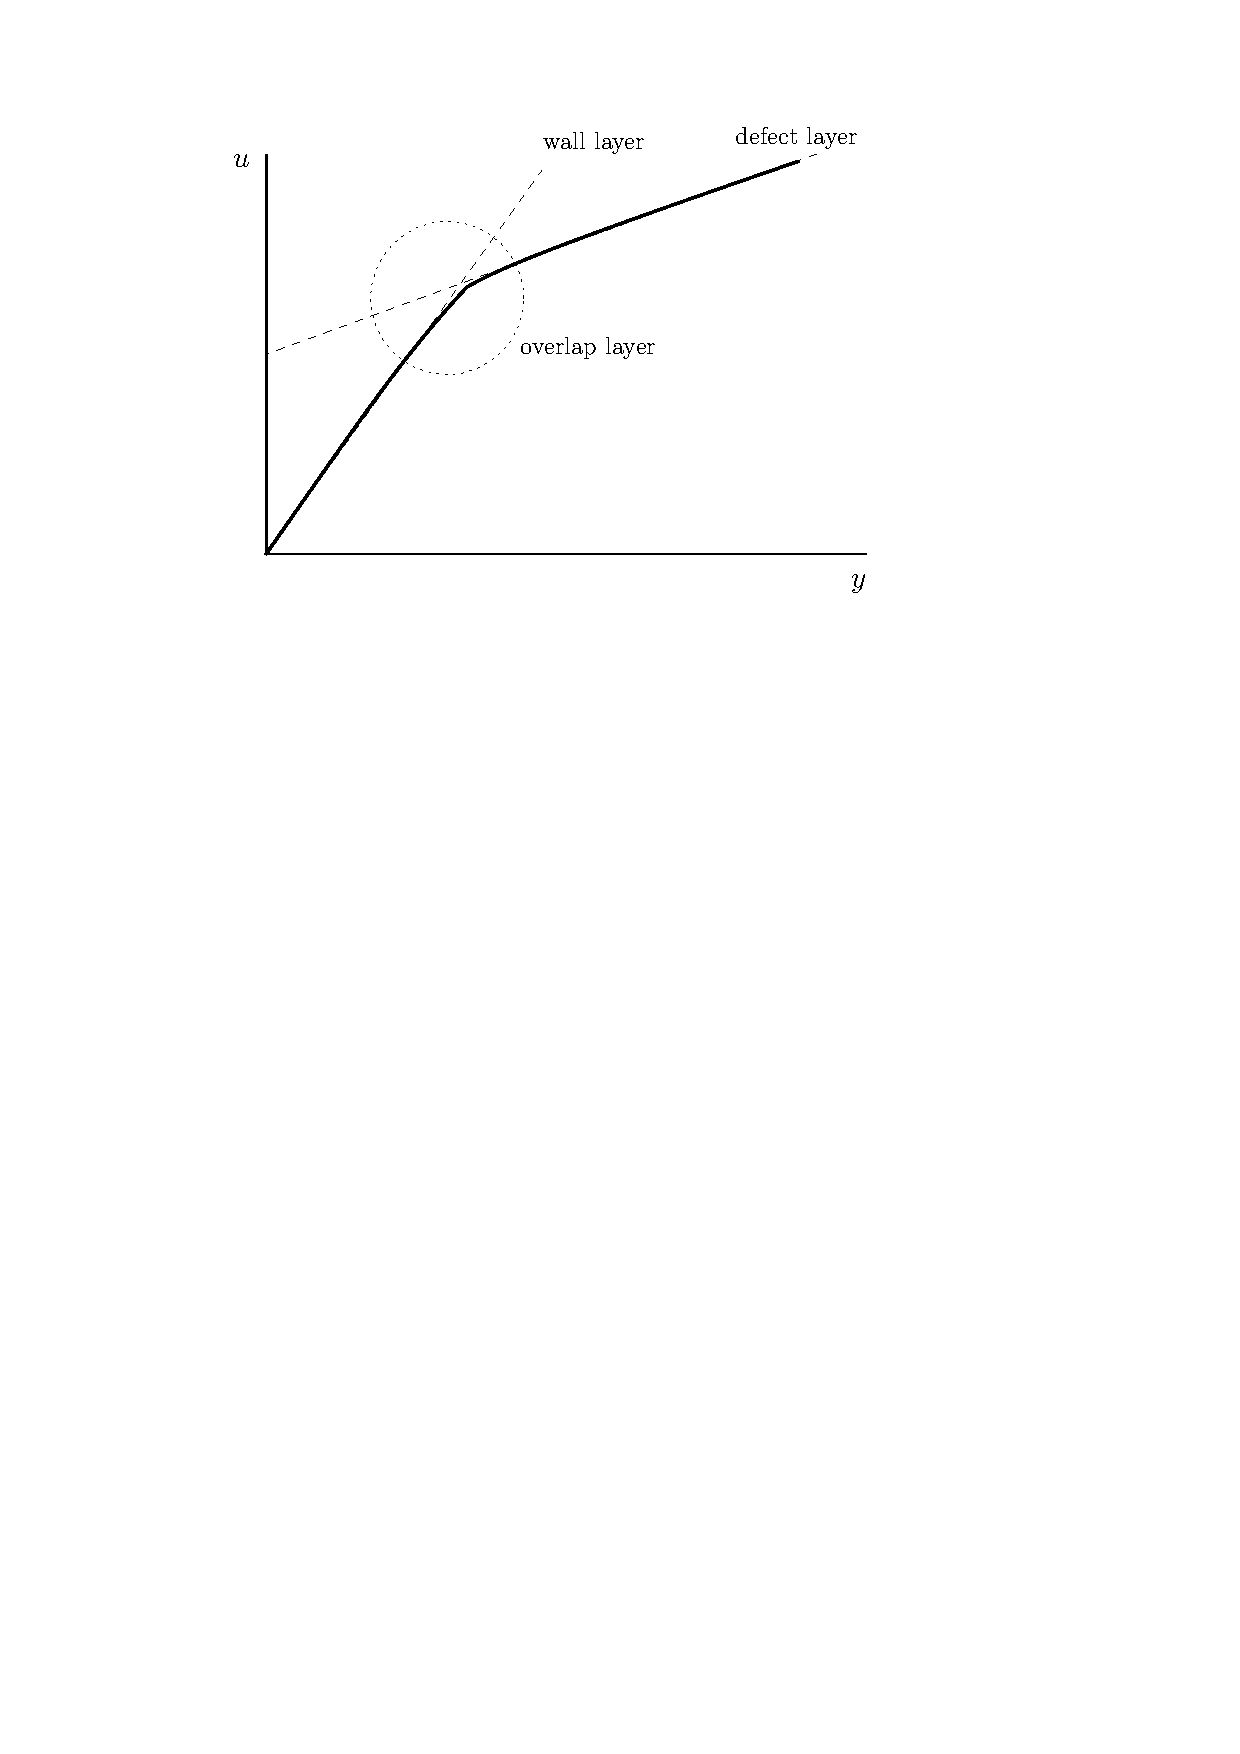
\includegraphics[scale=0.6]{./8.3 Profili di velocità/8.3-1}
		\centering
		\caption{Overlap layer}
	\end{figure}
%

Data la G, le due funzioni per wall e defect layer valgono purché siano vere delle condizioni:
%
	\begin{equation*}
		\begin{gathered}
			G\left( \frac{y}{h}, \frac{y u_t}{\nu} \right)\\
			\text{F  ok se } \frac{y u_\tau}{\nu} >> 1\\  
			\text{f  ok se } \frac{y}{h} << 1
		\end{gathered}
	\end{equation*}
%
Si ha quindi un overlap nell'intervallo $\frac{\nu}{u_\tau} << y << h$.

Questo è possibile perché è un numero di Reynolds con $u_\tau$ e non $U$, deve essere grande poiché si è nel caso turbolento, in effetti $\frac{h u_\tau}{\nu}$ è grande, questo assicura dell'esistenza dell'overlap.
Nell'overlap le due espressioni devono essere circa uguali:
%
	\begin{equation*}
		f\left( \frac{y u_\tau}{\nu} \right) \approx \frac{U}{u_\tau} - F \left( \frac{y}{h} \right)
	\end{equation*}
%

%SUBSECTION
\subsection{Soluzione di Millikan}
Una soluzione al problema fu trovata da Millikan:
%
	\begin{equation*}
		\begin{gathered}
			a \log{\left( \frac{y u_\tau}{\nu} \right)} + b = \frac{U}{u_\tau} - A \log{\left( \frac{y}{h} \right)} - B\\
			a \log{y} + a \log{\left( \frac{u_\tau}{\nu} \right)} + b = \frac{U}{u_\tau} - A \log{y} + A \log{h} - B
		\end{gathered}
	\end{equation*}
%
Si arriva quindi a queste condizioni:
%
	\begin{equation*}
		\begin{gathered}
			a = -A\\
			a \log{\left( \frac{u_\tau}{\nu} \right)} + b = \frac{U}{u_\tau} + A \log{h} - B
		\end{gathered}
	\end{equation*}
%
Per notazione si introduce $\kappa$, la costante di Von Karman:
%
	\begin{equation*}
		\begin{gathered}
			a = \frac{1}{k}\\
			k \sim 0.39
		\end{gathered}
	\end{equation*}
%
Mettendo assieme il tutto:
%
	\begin{equation*}
		\frac{U}{u_\tau} = \frac{1}{k} \log{\left( \frac{h u_\tau}{\nu} \right)} + b + B
	\end{equation*}
%

Si riprende poi la differenza tra il numero di Reynolds ``normale'' (alias bulk) e quello calcolato con lo sforzo:
%
	\begin{equation*}
		\begin{gathered}
			R_e \equiv \frac{2 h \bar{u}}{\nu}\\
			R_{e \tau} \equiv \frac{h u_\tau}{\nu}
		\end{gathered}
	\end{equation*}
%
Ricordando il coefficiente d'attrito/friction coefficient:
%
	\begin{equation*}
		C_f \equiv \frac{\tau_w}{\rho \bar{u}^2/2} = \frac{\rho u^2_\tau}{\rho \frac{\bar{u}^2}{2} } = 2 {\left( \frac{u_\tau}{\bar{u}} \right)}^2
	\end{equation*}
%
Si arriva finalmente a:
%
	\begin{equation*}
		\bar{u} = \frac{1}{h} \int_0^h u \dd{y} = \frac{1}{h} \int_0^h \left[ U - u_\tau F \left( \frac{y}{h} \right) \right] \dd{y}
	\end{equation*}
%
Quindi:
%
	\begin{equation*}
		\begin{gathered}
			\bar{u} = U - u_\tau \int_0^h F \left( \frac{y}{h} \right) \frac{\dd{y}}{h} = U - C u_\tau\\
			\text{Sostituendo}\\
			\frac{\bar{u}}{u_\tau} = \frac{1}{\kappa} \log{\left( \frac{h u_\tau}{\nu} \right)} + b +B -C
		\end{gathered}
	\end{equation*}
%
Raggruppando le costanti e inserendo $R_{e \tau} = \frac{u_\tau}{2 \bar{u}} R_e$:
%
	\begin{equation*}
		\begin{gathered}
			\sqrt{\frac{2}{C_F}} = \frac{1}{\kappa} \log{R_{e \tau}} + D =\\
			= \frac{1}{k} \log{\left( \frac{1}{2} \sqrt{\frac{C_F}{2}} R_e \right)} + D
		\end{gathered}
	\end{equation*}
%
Non è invertibile ma è possibile trovare graficamente $C_f$
%
	\begin{figure}[ht]
		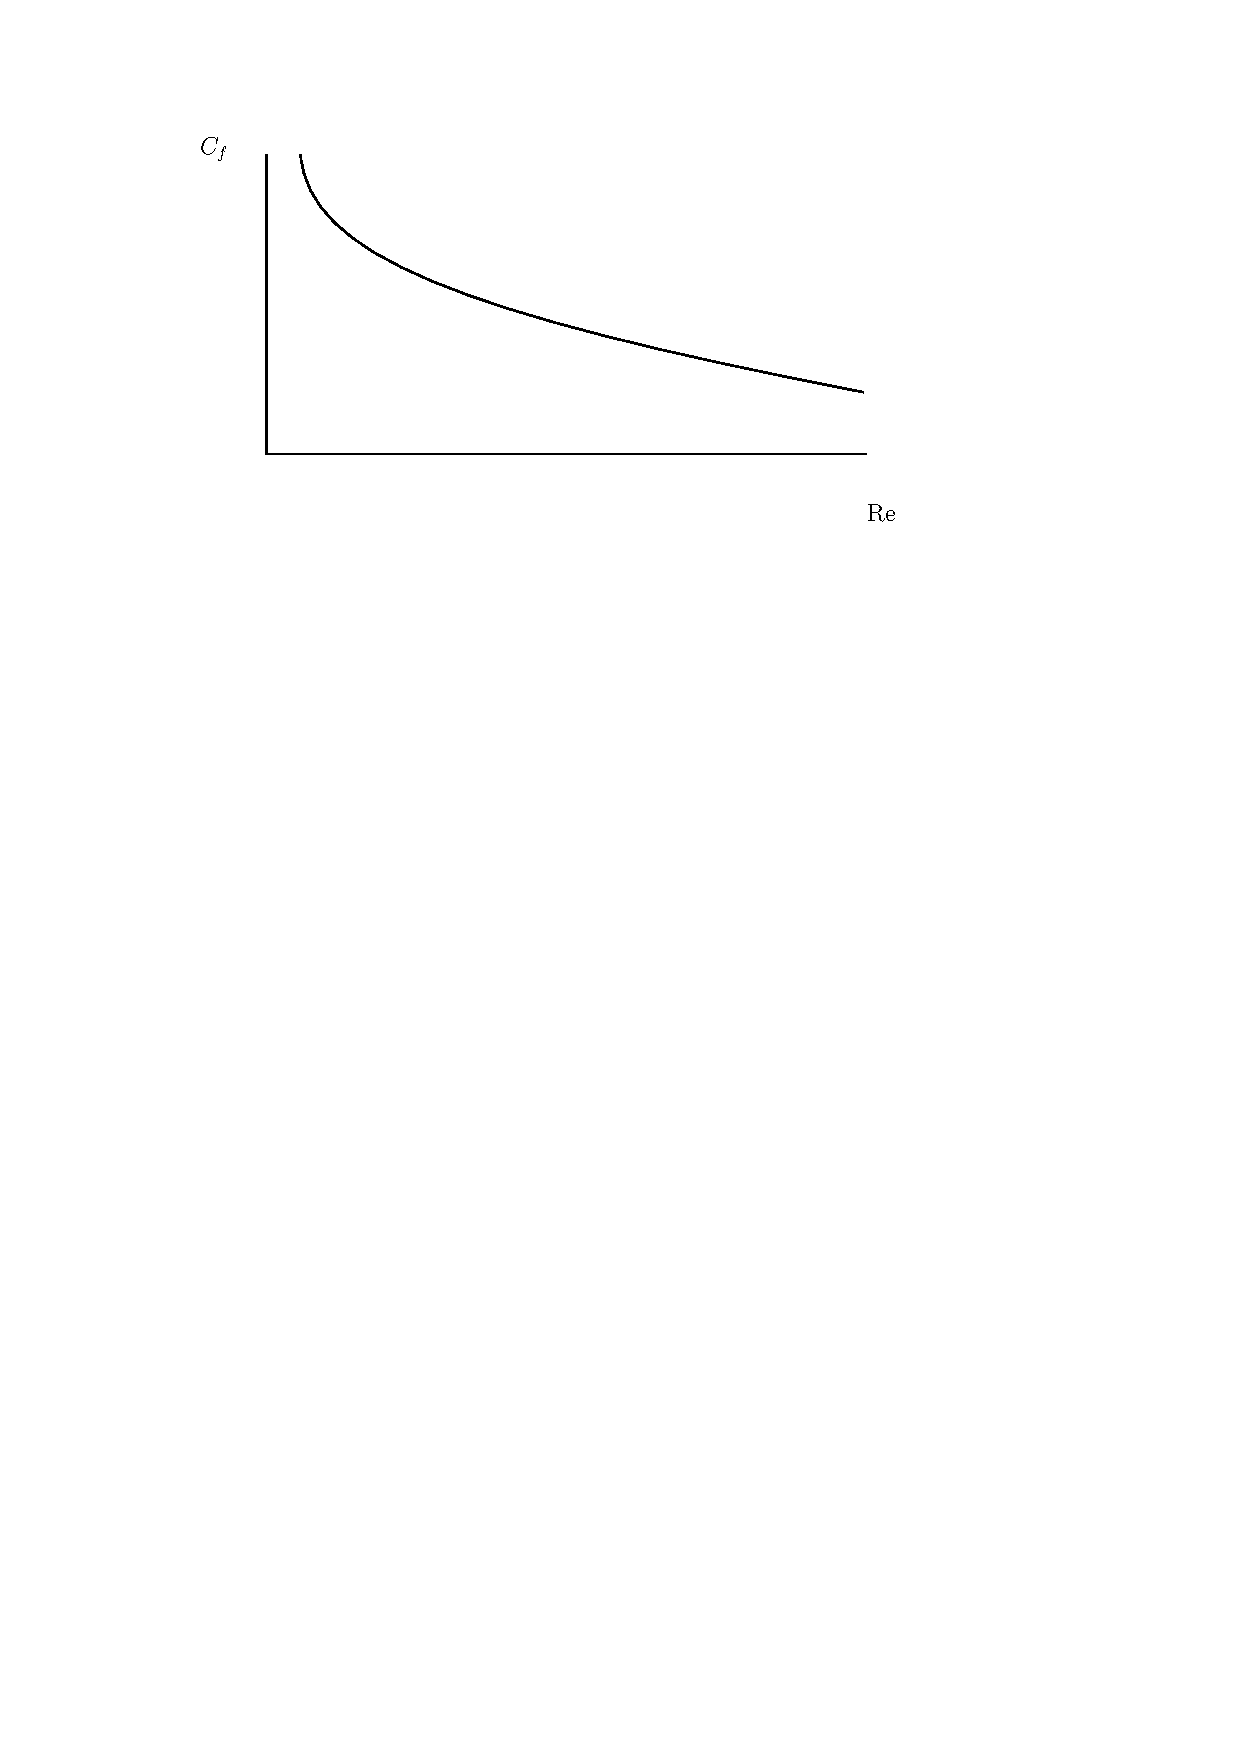
\includegraphics[scale=0.7]{./8.3 Profili di velocità/8.3-2}
		\centering
		\caption{Diagramma di Moody}
	\end{figure}
%

Un altro modo di rappresentare la velocità è il seguente.
Nel viscous sublayer:
%
	\begin{equation*}
		\begin{gathered}
			u^+ = \frac{u}{u_t} = f\\
			u = \frac{\tau}{\mu_2} y\\
			u = \frac{u_t}{\nu} y \\
			u^+ = y^+
		\end{gathered}
	\end{equation*}
%

Quindi si può rappresentare:
 %
	\begin{figure}[ht]
		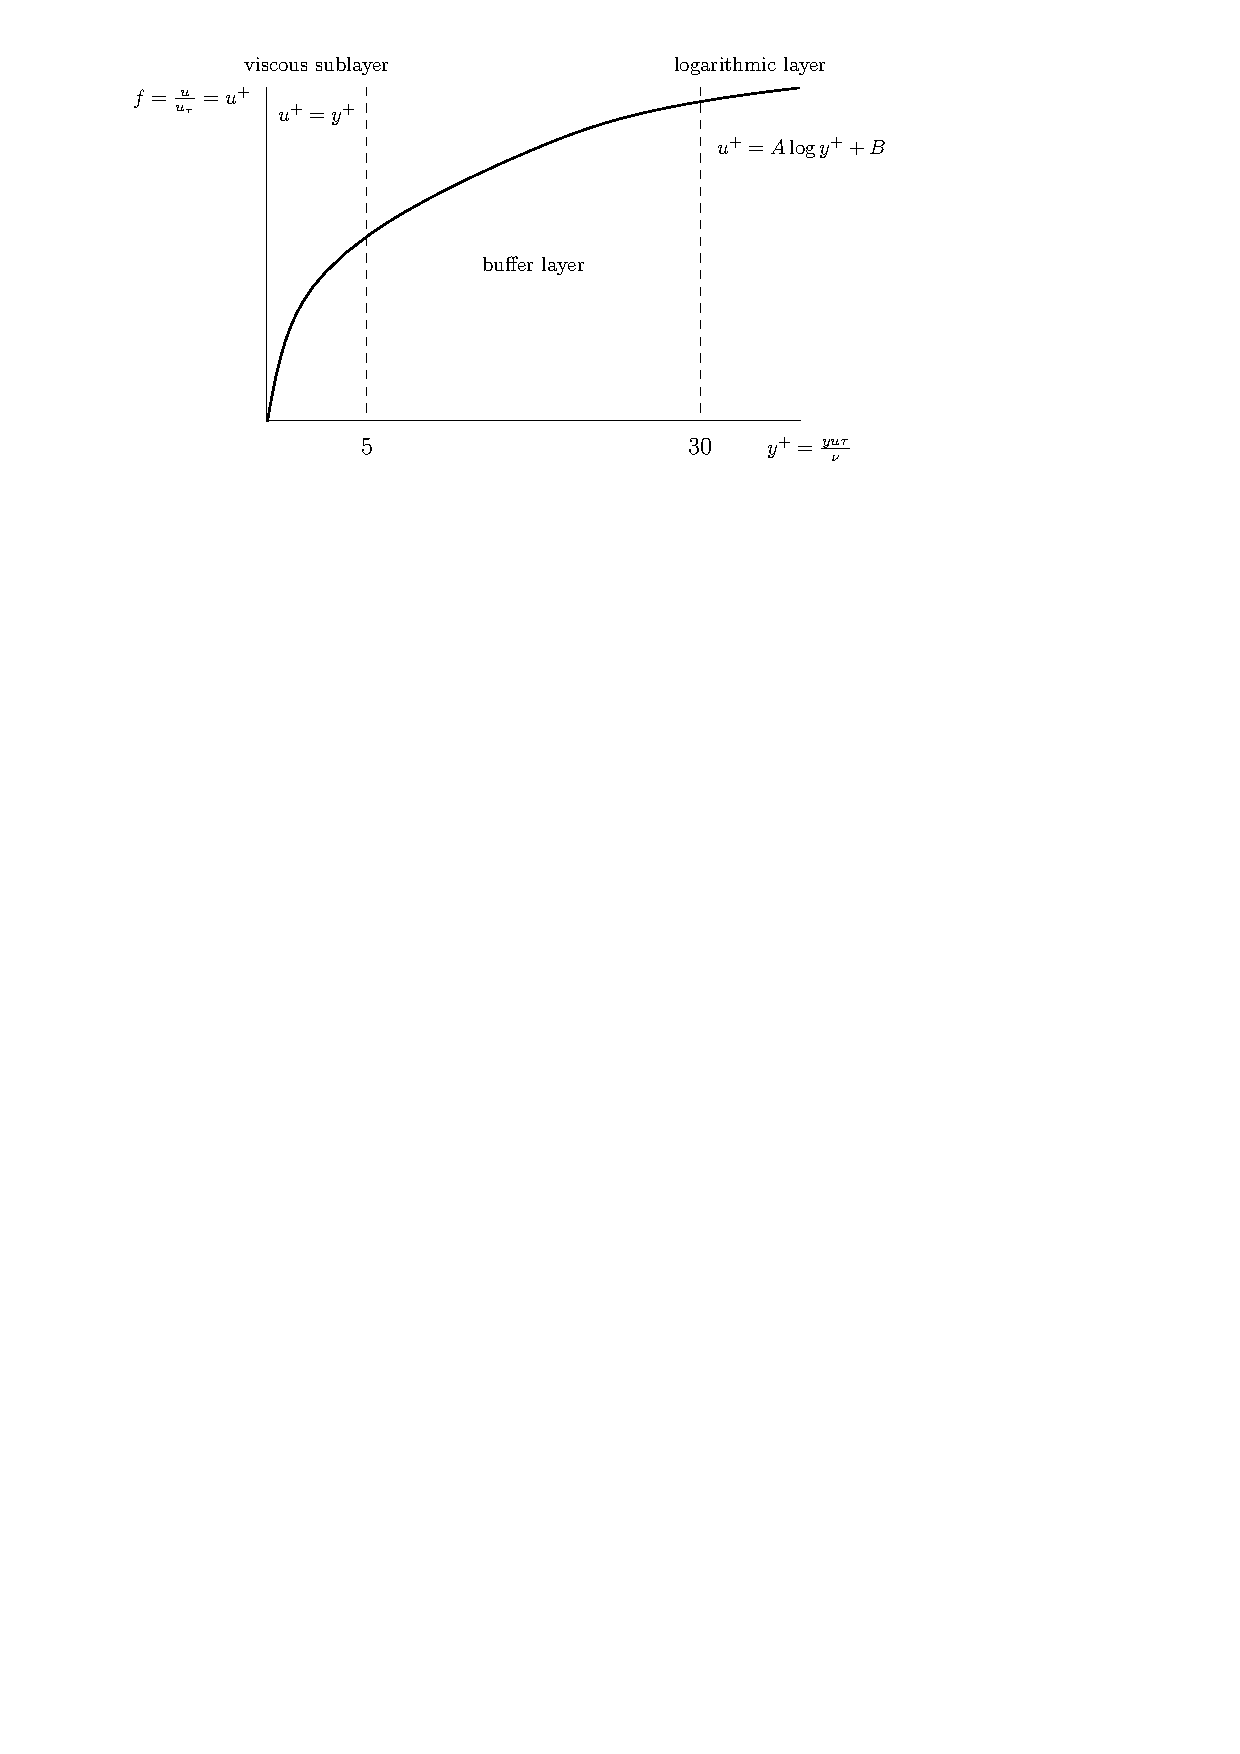
\includegraphics[scale=0.7]{./8.3 Profili di velocità/8.3-3}
		\centering
		\caption{Profilo di velocità}
	\end{figure}
% 


\subsection*{Bibliografia 8.3}
\cite[Cap.\ 12.4, 12.5]{PnueliGutfinger}